\section{Introduction}
% no \IEEEPARstart
Snake-like robots, with multiple joints and degree of freedom, 
have strong mobility in complex and unknown terrains\cite{Chirikjian1995The}. 
Therefore, they can complete tasks in many occasions, such as disaster 
rescuing\cite{DogAndSnake}, factory pipe maintenance\cite{ACMTutorial} 
and scientific exploration\cite{Kuwada2007Snake}. In the past decades, 
with the advent of orthogonal and universal joint structure\cite{1014757}\cite{Date2005Control}\cite{GaitBasedCompliant}, 
snake-like robots acquired the ability of three-dimensional space movement, 
which strengthens their mobility in varied topography. 

Although the snake-like robots have high mobility in many environments, the control of snake-like robots is complicated. A variety of motions can be constructed to get the same motion effect in the same environment because of the features of snake-like robots like multiple joints and degree of freedom. Moreover, the movements of snake-like robots are difficult to be predefined or inferred in the unknown environment.

Nowadays, based on a widely used motion model\cite{HiroseSine} of snake-like robots, we can pre-define the parameters to make robots move correctly in the known environment. However, this method is not feasible for the unknown environment. In unknown environments, tunning parameters artifically is inefficient because tunning the parameters inaccurately will break the motion of snake-like robots and it is difficult to tune the parameter accurately during robots' motion. In addition, controlling the robots is a professional work. Therefore, autonomous mobility of robots is an expectation in robots' motion.
%Although the snake-like robots have high mobility in many environments, the movement of most snake-like robots in unknown environments is directly controlled by human, reducing the efficiency and limiting the implementation of snake-like robots. Therefore, it is an important and challenging task to give them the ability to move in complex environment without real-time human intervention, that is, the autonomous mobility.

Autonomous mobility is an important and challenging task in robots' adaptability to environments. It is quite tough for programmer to take full account of all possible scenarios and have a good understanding of the interaction between the robot and the environment to construct a behavior-based autonomous model for robots, which increases the programmer's programming intensity and makes a weak effect on the movement in the unknown and mutational environment as well as has a weak adaptability to the environment.

In this paper, we propose a novel experience-based control strategy,
which autonomously determines the optimal control parameters of a snake-like robot in
current environment by entropy variance\cite{WaveformEntropyVariance}\cite{EntropyandVarianceasRiskMeasure}\cite{UsingEntropyAndVariance}. By tunning the optimal control parameter with regression value through the weighted least squares algorithm\cite{gradientMethod}\cite{MSEestimates}, we achieve to make the robot gradually adapt itselt to the environment. The whole process of our control strategy can be divided into two parts:
\begin{enumerate}
	\item data acquisition and preprocessing,
	\item real-time data feedback and multi-parameter regression control.
\end{enumerate}
\begin{figure}[!t]
	\centering
	\subfigure[Reality robot]{
		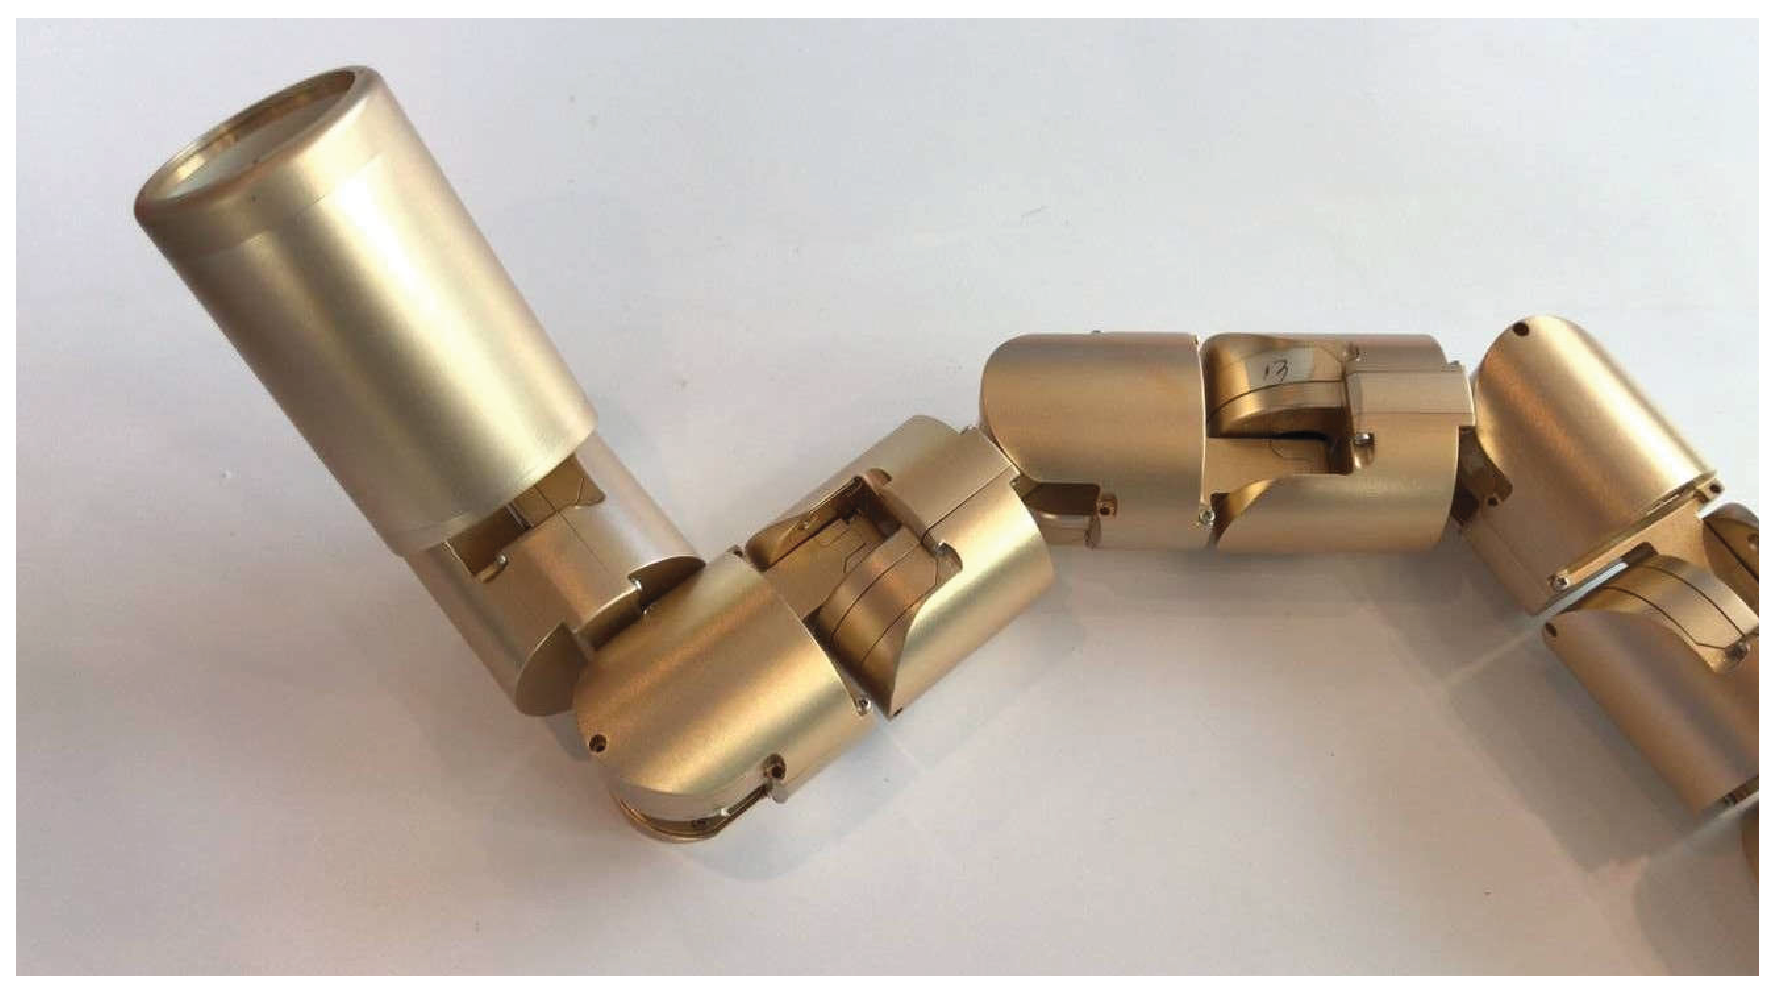
\includegraphics[width=1.5in,height=0.75in]{fig/relative/realSnake}
		\figlabel{fig:snake_like_robot_a}
	}
	\subfigure[Simulation robot]{
		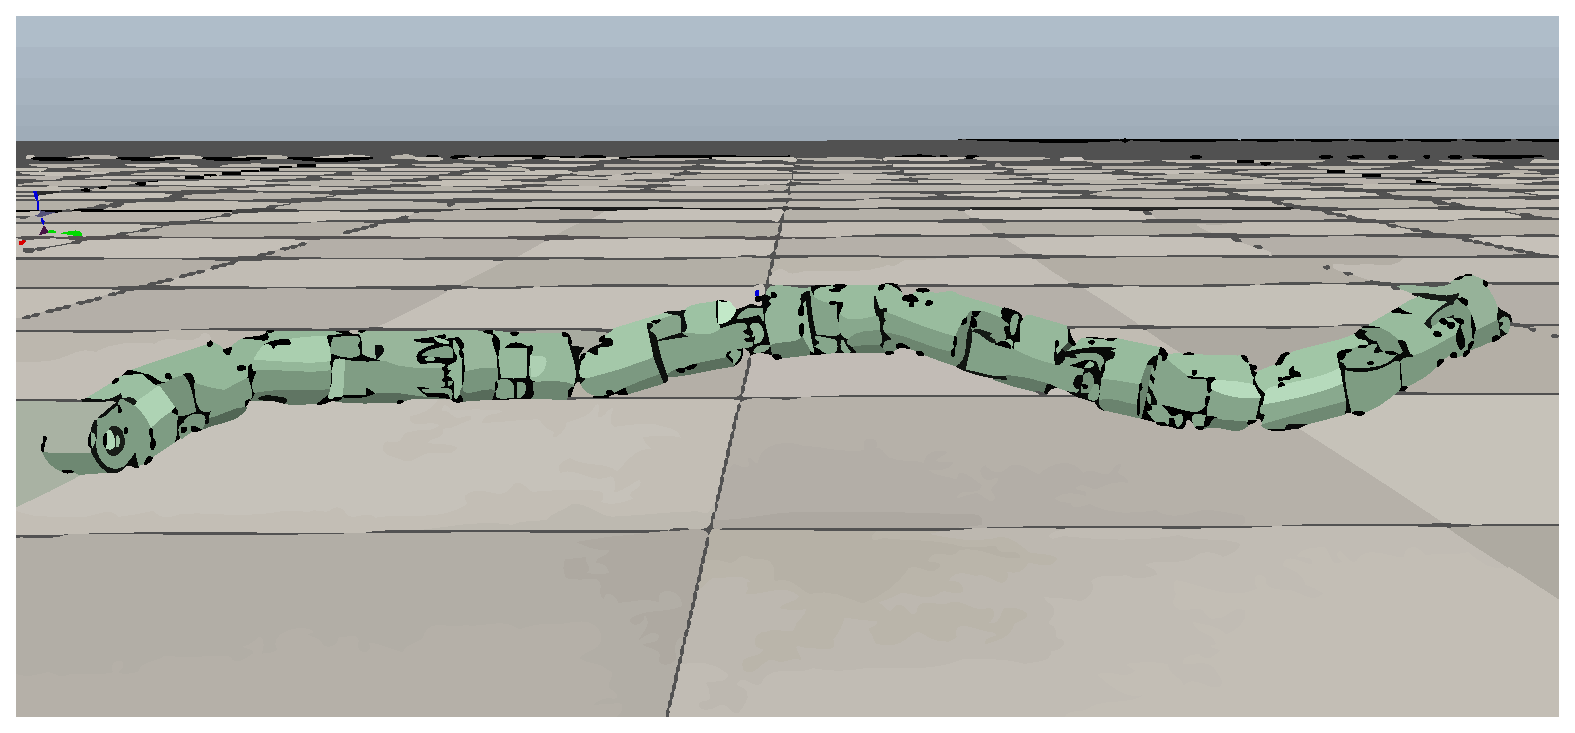
\includegraphics[width=1.5in,height=0.75in]{fig/relative/simulateSnake}
		\figlabel{fig:snake_like_robot_b}
	}
	\caption{The Snake-like robot}
	\figlabel{fig:snake_like_robot}
\end{figure}
%In the first part, we collect data that reflecting the dynamic states of a snake-like robot in varies environments and then form a training set. The clustering algorithm\cite{Cluseter_ICT}\cite{KmeansAndDeepLearning} is adopted in this part to reduce the time overhead of feed-back control. In the second part, we apply regression and feed-back control based on previous training data of the motion of robots. The multi-parameter regression is also transformed into an unit regression problem for higher efficiency. We adopt the entropy variance\cite{WaveformEntropyVariance}\cite{EntropyandVarianceasRiskMeasure}\cite{UsingEntropyAndVariance} as the criterion for accessing the effect of the control parameters on the motion. Then the most sensitive parameter which has the greatest effect on motion is selected to perform the unit regression. By transforming the multiple regression into the  unit regression and combining the weighted least squares algorithm\cite{gradientMethod}\cite{MSEestimates},  we finally get a fitted regression function and obtain the value of the optimal parameter.
To evaluate the effectiveness of the proposed framework, we also apply it to the our 
existing snake-like robot platform, which is shown in~\figref{fig:snake_like_robot_a}
and~\figref{fig:snake_like_robot_b}. Under our framework, the robot climbs pipes having different diameters and the
performance of climbing is reported. In summary, the contributions of this paper are:
\begin{itemize}
	\item A new framework for robot adaptive control is proposed.
 	      This framework greatly reduces the amount of  effort of the regression calculation 
           by adopting clustering algorithm for data preprocessing and the classification of 
           real-time data.
	\item A transformation of multiple regression problem is proposed to obtain the optimal
          control parameters in a real-time manner.
         The entropy variance is utilized to select the parameter which is the most sensitive 
         in current state. Then, by regressing this parameter instead of all the parameters, the 
         multiple regression is transformed into an unit regression problem.
    \item A set of case studies is conducted and the results demonstrate
    that our proposed strategy is effectiveness in accomplishing autonomous movement for snake-like robots.
\end{itemize}
%The robot has an orthogonal structure with 18 joints. Each joint has a rotation axis which
%is perpendicular to the body. The rotation axes of two adjacent joints are orthogonal with each other,
%thus forming a three-dimensional space movement. a set of sensors such as accelerometer and gyro
%is embedded in each joint to realize the feedback control.

The rest of this paper is organised as follows. Early preparations are demonstrated in the Section \uppercase\expandafter{\romannumeral2}. In Section \uppercase\expandafter{\romannumeral3}, proposed strategy is explained in detailed. And then Simulation works are illustrated in Section \uppercase\expandafter{\romannumeral4}. Section \uppercase\expandafter{\romannumeral5} shows the conclusion and our future prospects about the proposed strategy.

%The simulation environment is the pipe climbing, which can be used in cable detection of cable-stayed bridge. In the first part, we collect data in pipes with different diameter as training set. To reduce time of calculation in feed-back control, we adopt clustering algorithm\cite{Cluseter_ICT}\cite{KmeansAndDeepLearning}. In the second part, we apply regression and feed-back control based on previous training data on the motion of robots. We utilize the entropy variance\cite{WaveformEntropyVariance}\cite{EntropyandVarianceasRiskMeasure}\cite{UsingEntropyAndVariance} to measure the effect of the control parameters on the motion and select the most sensitive parameter which has the greatest effect on motion. By transforming the multiple regression into the unit regression and combining the weighted least squares algorithm\cite{gradientMethod}\cite{MSEestimates}, we finally get a fitted regression function and modify the most sensitive parameter.